
\section{Functional Requirements}

We have to develop various pieces of code to materalize this project that ranges from collecting data to representing PPIN as networks using libraries such \texttt{Networkx, iGraph, Numpy, Matplotlib, Pandas} to running large analysis algorithms through the help of various libraries such as \texttt{Tensorflow, Scikit-Learn}. 

Furthermore, we will implement our own classes and methods in \texttt{Python} that will serve various purposes and and will work in-tandem. These will be comprised of wrapping the above mentioned libraries and their methods, and other other open source bioinformatics libraries such as PyBioMed \cite{dong_pybiomed_2018}. A functional hierarchy of all of our final work may look like:
\begin{outline}
  \1 \texttt{Data API}
%   \2 Function 1:
%   \2 Function 2:
  \1 \texttt{PPIN Class}
%   \2 Function 1:
%   \2 Function 2:
  \1 \texttt{Analysis Class}
  \1 \texttt{Prediction Class}
  \1 \texttt{Visualization API}
\end{outline}

% --- The above is to be modified as per your project, e.g. a flat list if your system has limited functional requirements.

% \section{Non-functional Requirements}

% This sections mentions the specific non-functional requirements of our system. These generally address performance, scalability, safety, availability, deployment etc.


\section{External Interfaces}

\subsection{Visualization}
To visualize the protein-protein interactions (PPI), we will potentially be using a software, like PyMol. PyMol is a 3D protein visualizer software that can visualize single proteins and could also used to show the PPI. Figure 3.1 shows a 3D protein-ligand interaction that we did manually to depict what our potential final deliverable would look like. The input for the protein files would in the form of a Protein Data Bank (PDB) ID. We would get these files as a result of the protein clusters that we get from the clustering algorithms from the ensemble framework.
\begin{figure}[h!]
\centering
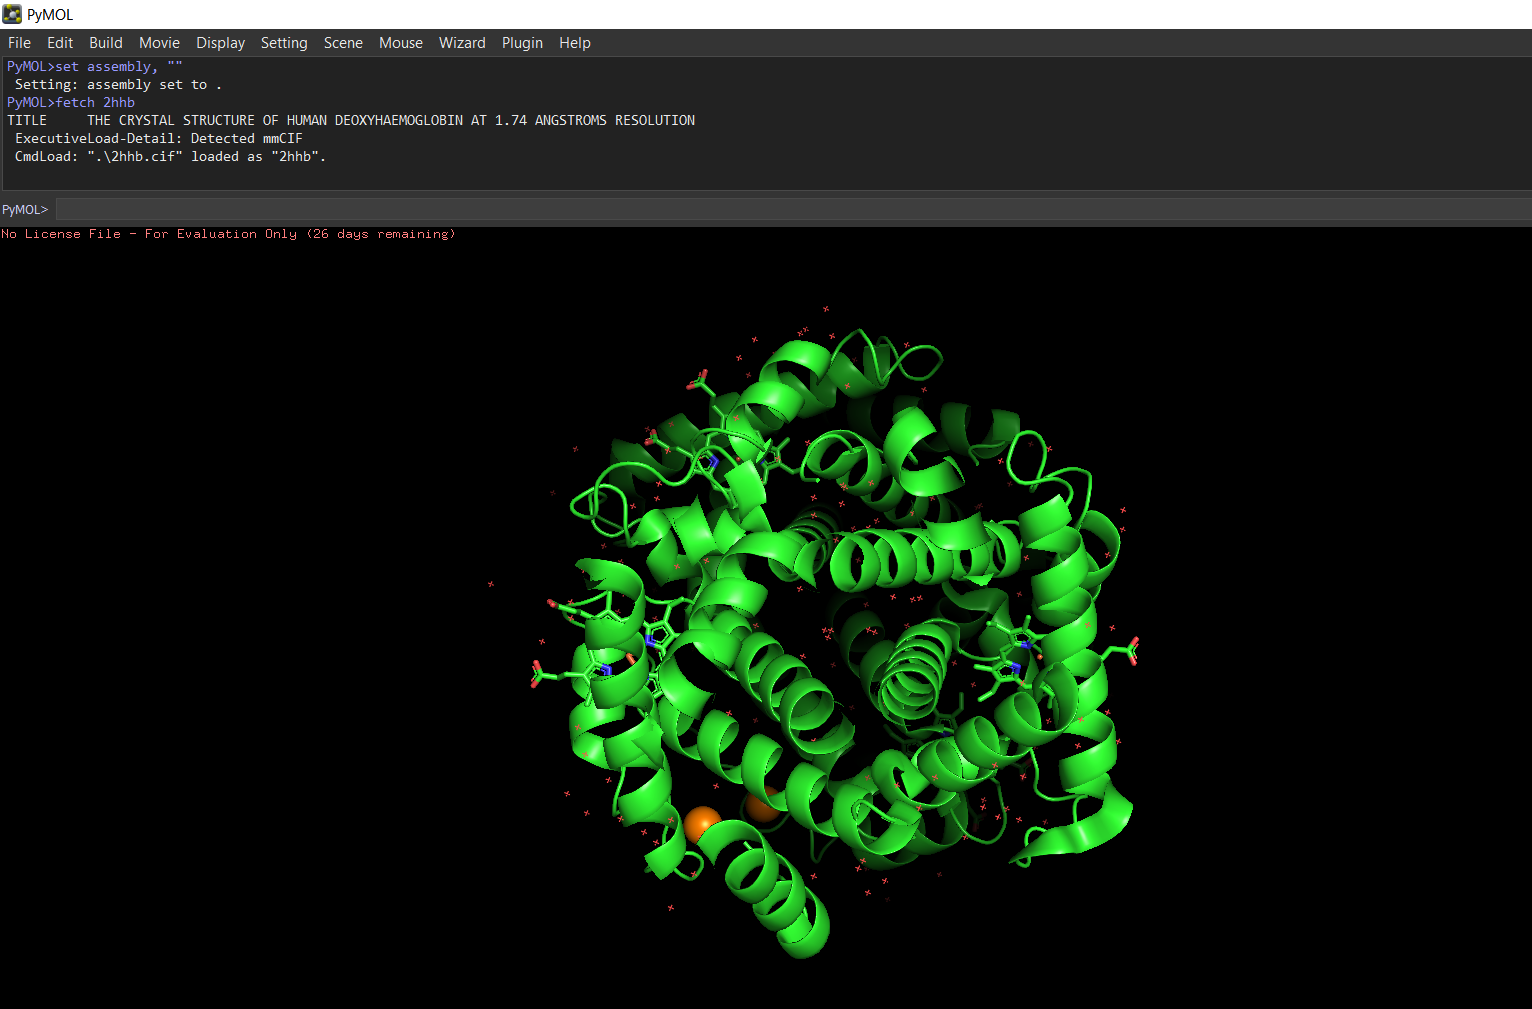
\includegraphics[scale=0.5]{./PyMol.png}
\caption{Protein-Ligand Interaction}
\label{fig:PyMol}
\end{figure}

\section{Datasets}
% This section describes the specific dataset(s) used to build our system. An appropriate snapshot of the dataset(s) is also included. Futher details, when needed, are presented in the appendix.
The collection and compilation of datasets to form a complete database of protein-protein interaction networks (PPIN) is an integral part of the project. The datasets used in our project are centered around one singular species; \textit{homo sapiens}, without any restriction on the list of proteins forming the global network. The datasets are extracted from online repositories such as BioGRID, APID, STRING that collect data about protein protein interactions from biological and bio-informatic literature. 

% \subsection{Purpose}

\subsection{PPIN Datasets}
The PPIN datasets that the project will work with will be from a singular species; \textit{homo sapiens}, as mentioned earlier and will be extracted from multiple online repositories. The data preserved in these datasets will be in a pairwise format where each row stores information such as the \textit{uniProtKB} and name of each protein in a protein-protein interaction pair, along with the MINT score of the interaction.\\\\
The information for each column entry in the dataset is as follows:
\begin{itemize}
    \item \textbf{UniProtKB ID:} The uniProtKB of a protein is the unique primary identifier of an interactor stored in the uniProt database. It is an ID assigned to a protein interactor for identification within uniProt and is considered universal.\\
    There will be two columns of UniProt IDs(UniProtA and UniProtB), one for each protein interactor (in this case protein A and protein B) in a protein-protein interaction pair.
    \item \textbf{Gene Name:} The recommended name used to officially represent any gene, adhering to the gene nomenclature.\\
    There will be two columns of Gene Names (GeneName A and GeneName B), one for each protein interactor (in this case protein A and protein B) in a protein-protein interaction pair.
    \item \textbf{Score:} The score assigned to any interaction pair is a value between 0 and 1 that is representative of all the cumulative experimental evidence of an existing interaction between the two interactors, as retrieved from multiple different databases. The score is calculated by using the MINT scoring function given as follows:
    $$S = 1-a^{-x}$$
    where, $a$ represents the initial slope of the curve and is arbitrarily chosen and $x$ represents the combined experimental evidence, and is obtained by summing up experimental evidence weighted by coefficients $d$ and $e$, which cater to the size of the experiment and method of experimentation respectively. $x$ can be given as follows:
    $$x = \sum_{i}d_{i}e{i} + \frac{n}{10}$$
    In the function above, $n$ represents the number of publications that give supporting evidence for existence of the interaction.
    The MINT score ensures that only those interactions supported by multiple experimental techniques and publications have a score close to 1 and those that lack sufficient evidence have a lower score. 
\end{itemize}


% \subsection{Protein Data}
\subsection{Table of Datasets}
The list of sources or online repositories from which the data will be extracted is given as follows:
\begin{table}[htpb]
      \centering
      \caption{A list of PPI databases.}
      \vspace{1 em}
      \label{tab:dataset1}
      \begin{tabular}{l|l}
      \hline
      Name & Website \\
      \hline
      DIP & \url{http://dip.doe-mbi.ucla.edu/dip/Main.cgi}\\
      BioGRID & \url{https://thebiogrid.org/} \\
      APID & \url{http://cicblade.dep.usal.es:8080/APID/init.action}\\
      HPRD & \url{http://www.hprd.org/} \\ 
      MINT & \url{https://mint.bio.uniroma2.it}\\
    STRING & \url{https://string-db.org/} \\
    \hline
    \end{tabular}
  \end{table}

\subsection{Method for Compilation}
The acquisition of datasets and compilation of the datasets is an integral part of the formation of a usable database. The datasets will firstly be collected by running a query on the online repositories which extracts all possible PPIN for human proteins such as GRB2.\\\\The key challenge then presents itself in the form of the compilation of the datasets, where each extracted and downloaded dataset is in a different format in terms of how the data is presented as well as the type of data that is presented. Some data does not have the MINT score included which can then be confirmed by running a query on the MINT repository or on MENTHA.\\\\
The datasets are first be converted into a standardized readable format, preferably in the form of a TSV. The data within will then be standardized in terms of the presentation of the data. The standardized datasets will then be compiled and filtered to remove incomplete or multiple instances of the data. The steps are highlighted in the compilation pipeline given in the diagram below.
\begin{figure}[h!]
    \centering
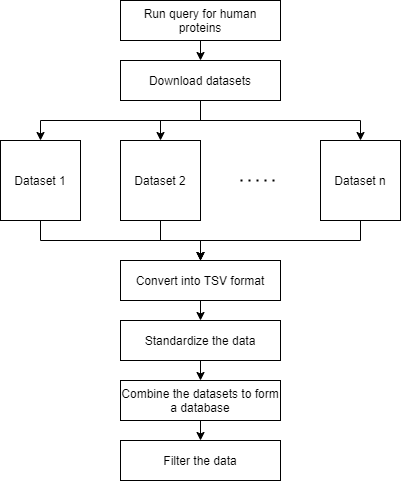
\includegraphics[scale=1]{Final-Report-Kavish-1/chapters/compilation-pipeline.drawio.png}
\caption{Compilation Pipeline.}
\end{figure}


% \begin{enumerate}
%     \item The online repositories will be queried for human proteins such as GRB2
%     \item The datasets will be downloaded and converted into TSV format
%     \item 
% \end{enumerate}
% \subsection{Interfacing with Dataset}

% \section{System Diagram}
% This diagram gives a high-level view of the different components of our system and the interactions between them. Each component and the particular tools/technologies/libraries used to build it are described.